\appendix\label{ch:Appendix}

%In this appendix, the flavour-tagging performance for different geometries, jet polar angles and energies are shown.

\newcounter{energy}     
\section{Flavour tagging and jet-angle dependence for the CDR geometry}\label{sec:CDR_jet_angle}       
\foreach \energy in {1000, 500, 200, 91}
{%
        \setcounter{energy}{\energy}
               \subsection{Jets in dijet events at $\sqrt{s}=$\arabic{energy}~GeV}\label{sec:\arabic{energy}}
                \begin{figure}[H]              
                  \begin{subfigure}[b]{0.5\textwidth}
                 \centering
                   \begin{tikzpicture}
                   \node[anchor=south west,inner sep=0] (image) at (0,0){\includegraphics[width=\textwidth]{Figures/ImpactOfGeometries/allAngles_CLIC_SiD_CDR_Beauty_Charm_\arabic{energy}.pdf}};
                   \draw[white, fill=white] (1.8, 6.3) rectangle (5.7, 7);
                   \end{tikzpicture}
                 \caption{}
                  \label{}
                  \end{subfigure}%
                  ~ 
                  \begin{subfigure}[b]{0.5\textwidth}
                  \centering
                  \begin{tikzpicture}
                   \node[anchor=south west,inner sep=0] (image) at (0,0){\includegraphics[width=\textwidth]{Figures/ImpactOfGeometries/allAngles_CLIC_SiD_CDR_Beauty_LF_\arabic{energy}.pdf}};
                  \draw[white, fill=white] (1.8, 6.3) rectangle (5.7, 7);
                   \end{tikzpicture}
                  \caption{}
                  \label{}
                  \end{subfigure}
                  \caption{b-tag efficiency for jets dijet events at $\sqrt{s}=$\arabic{energy}~GeV with different polar angles using the CDR geometry.}\label{}
                 \end{figure}

                 \begin{figure}[H]
                 \begin{subfigure}[b]{0.5\textwidth}
                 \centering
                 \begin{tikzpicture}
                   \node[anchor=south west,inner sep=0] (image) at (0,0){\includegraphics[width=\textwidth]{Figures/ImpactOfGeometries/allAngles_CLIC_SiD_CDR_Charm_Beauty_\arabic{energy}.pdf}};
                  \draw[white, fill=white] (1.8, 6.3) rectangle (5.7, 7);
                   \end{tikzpicture}
                    \caption{}
                    \label{}
                   \end{subfigure}%
                       ~ 
               \begin{subfigure}[b]{0.5\textwidth}
                  \centering
                 \begin{tikzpicture}
                   \node[anchor=south west,inner sep=0] (image) at (0,0){\includegraphics[width=\textwidth]{Figures/ImpactOfGeometries/allAngles_CLIC_SiD_CDR_Charm_LF_\arabic{energy}.pdf}};
                  \draw[white, fill=white] (1.8, 6.3) rectangle (5.7, 7);
                   \end{tikzpicture}
                 \caption{}
               \label{}
            \end{subfigure}
              \caption{c-tag efficiency for jets in dijet events at $\sqrt{s}=$\arabic{energy}~GeV with different polar angles using the CDR geometry.}\label{}
            \end{figure}

}%

\section{Flavour tagging and jet-angle dependence for the \emph{spirals} geometry}\label{sec:spirals_jet_angle}       
\foreach \energy in {1000, 500, 200, 91}%, 500, 200, 91}
{%
        \setcounter{energy}{\energy}
               \subsection{Jets in dijet events at $\sqrt{s}=$\arabic{energy}~GeV}\label{sec:\arabic{energy}}
                \begin{figure}[H]              
                  \begin{subfigure}[b]{0.5\textwidth}
                 \centering
                 \begin{tikzpicture}
                   \node[anchor=south west,inner sep=0] (image) at (0,0){\includegraphics[width=\textwidth]{Figures/ImpactOfGeometries/allAngles_CLIC_SiD_spirals_Beauty_Charm_\arabic{energy}.pdf}};
                  \draw[white, fill=white] (1.8, 6.3) rectangle (5.7, 7);
                   \end{tikzpicture}
                 \caption{}
                  \label{}
                  \end{subfigure}%
                  ~ 
                  \begin{subfigure}[b]{0.5\textwidth}
                  \centering
                  \begin{tikzpicture}
                   \node[anchor=south west,inner sep=0] (image) at (0,0){\includegraphics[width=\textwidth]{Figures/ImpactOfGeometries/allAngles_CLIC_SiD_spirals_Beauty_LF_\arabic{energy}.pdf}};
                  \draw[white, fill=white] (1.8, 6.3) rectangle (5.7, 7);
                   \end{tikzpicture}
                  \caption{}
                  \label{}
                  \end{subfigure}
                  \caption{b-tag efficiency for jets in dijet events at $\sqrt{s}=$\arabic{energy}~GeV with different polar angles using the \textit{spirals} geometry.}\label{}
                 \end{figure}

                 \begin{figure}[H]
                 \begin{subfigure}[b]{0.5\textwidth}
                 \centering
                 \begin{tikzpicture}
                   \node[anchor=south west,inner sep=0] (image) at (0,0){\includegraphics[width=\textwidth]{Figures/ImpactOfGeometries/allAngles_CLIC_SiD_spirals_Charm_Beauty_\arabic{energy}.pdf}};
                  \draw[white, fill=white] (1.8, 6.3) rectangle (5.7, 7);
                   \end{tikzpicture}
                    \caption{}
                    \label{}
                   \end{subfigure}%
                       ~ 
               \begin{subfigure}[b]{0.5\textwidth}
                  \centering
                 \begin{tikzpicture}
                   \node[anchor=south west,inner sep=0] (image) at (0,0){\includegraphics[width=\textwidth]{Figures/ImpactOfGeometries/allAngles_CLIC_SiD_spirals_Charm_LF_\arabic{energy}.pdf}};
                  \draw[white, fill=white] (1.8, 6.3) rectangle (5.7, 7);
                   \end{tikzpicture}
                 \caption{}
               \label{}
            \end{subfigure}
              \caption{c-tag efficiency for jets in dijet events at $\sqrt{s}=$\arabic{energy}~GeV with different polar angles using the \textit{spirals} geometry.}\label{}
            \end{figure}

}%

\section{Flavour tagging and jet-angle dependence for the \emph{double\_spirals} geometry}\label{sec:doubleSpirals_jet_angle}      
\foreach \energy in {1000, 500, 200, 91}%, 500, 200, 91}
{%
        \setcounter{energy}{\energy}
               \subsection{Jets in dijet events at $\sqrt{s}=$\arabic{energy}~GeV}\label{sec:\arabic{energy}}
                \begin{figure}[H]              
                  \begin{subfigure}[b]{0.5\textwidth}
                 \centering
                  \begin{tikzpicture}
                   \node[anchor=south west,inner sep=0] (image) at (0,0){\includegraphics[width=\textwidth]{Figures/ImpactOfGeometries/allAngles_CLIC_SiD_double_spirals_Beauty_Charm_\arabic{energy}.pdf}};
                  \draw[white, fill=white] (1.5, 6.3) rectangle (6.3, 7);
                   \end{tikzpicture}
                 \caption{}
                  \label{}
                  \end{subfigure}%
                  ~ 
                  \begin{subfigure}[b]{0.5\textwidth}
                  \centering
                  \begin{tikzpicture}
                   \node[anchor=south west,inner sep=0] (image) at (0,0){\includegraphics[width=\textwidth]{Figures/ImpactOfGeometries/allAngles_CLIC_SiD_double_spirals_Beauty_LF_\arabic{energy}.pdf}};
                  \draw[white, fill=white] (1.5, 6.3) rectangle (6.3, 7);
                   \end{tikzpicture}
                  \caption{}
                  \label{}
                  \end{subfigure}
                  \caption{b-tag efficiency for jets in dijet events at $\sqrt{s}=$\arabic{energy}~GeV with different polar angles using the \textit{double\_spirals} geometry.}\label{}
                 \end{figure}

                 \begin{figure}[H]
                 \begin{subfigure}[b]{0.5\textwidth}
                 \centering
                 \begin{tikzpicture}
                   \node[anchor=south west,inner sep=0] (image) at (0,0){\includegraphics[width=\textwidth]{Figures/ImpactOfGeometries/allAngles_CLIC_SiD_double_spirals_Charm_Beauty_\arabic{energy}.pdf}};
                 \draw[white, fill=white] (1.5, 6.3) rectangle (6.3, 7);
                   \end{tikzpicture}
                    \caption{}
                    \label{}
                   \end{subfigure}%
                       ~ 
               \begin{subfigure}[b]{0.5\textwidth}
                  \centering
                 \begin{tikzpicture}
                   \node[anchor=south west,inner sep=0] (image) at (0,0){\includegraphics[width=\textwidth]{Figures/ImpactOfGeometries/allAngles_CLIC_SiD_double_spirals_Charm_LF_\arabic{energy}.pdf}};
                 \draw[white, fill=white] (1.5, 6.3) rectangle (6.3, 7);
                   \end{tikzpicture}
                 \caption{}
               \label{}
            \end{subfigure}
              \caption{c-tag efficiency for jets in dijet events at $\sqrt{s}=$\arabic{energy}~GeV with different polar angles using the \textit{double\_spirals} geometry.}\label{}
            \end{figure}

}%

\section{\emph{spirals} vs. CDR}\label{sec:appendix_spirals_vs_CDR}   
\foreach \energy in {1000, 500, 200, 91}
{%
        \setcounter{energy}{\energy}
               \subsection{Jets in dijet events at $\sqrt{s}=$\arabic{energy}~GeV}\label{sec:\arabic{energy}}
                \begin{figure}[H]              
                  \begin{subfigure}[b]{0.5\textwidth}
                 \centering
                 \begin{tikzpicture}
                   \node[anchor=south west,inner sep=0] (image) at (0,0){\includegraphics[width=\textwidth]{Figures/ImpactOfGeometries/\arabic{energy}GeV_Ratio_allAngles_spirals_CDR_B_C.pdf}};
                 \draw[white, fill=white] (1.5, 6.3) rectangle (6.3, 7);
                   \end{tikzpicture}
                 \caption{}
                  \label{}
                  \end{subfigure}%
                  ~ 
                  \begin{subfigure}[b]{0.5\textwidth}
                  \centering
                  \begin{tikzpicture}
                   \node[anchor=south west,inner sep=0] (image) at (0,0){\includegraphics[width=\textwidth]{Figures/ImpactOfGeometries/\arabic{energy}GeV_Ratio_allAngles_spirals_CDR_B_LF.pdf}};
                 \draw[white, fill=white] (1.5, 6.3) rectangle (6.3, 7);
                   \end{tikzpicture}
                  \caption{}
                  \label{}
                  \end{subfigure}
                  \caption{b-tagging: the ratio between the misidentification probabilities for the \textit{spirals} and the CDR geometries based on jets in dijet events at $\sqrt{s}=$\arabic{energy}~GeV.}\label{}
                 \end{figure}

                 \begin{figure}[H]
                 \begin{subfigure}[b]{0.5\textwidth}
                 \centering
                 \begin{tikzpicture}
                   \node[anchor=south west,inner sep=0] (image) at (0,0){\includegraphics[width=\textwidth]{Figures/ImpactOfGeometries/\arabic{energy}GeV_Ratio_allAngles_spirals_CDR_C_B.pdf}};
                 \draw[white, fill=white] (1.5, 6.3) rectangle (6.3, 7);
                   \end{tikzpicture}
                    \caption{}
                    \label{}
                   \end{subfigure}%
                       ~ 
               \begin{subfigure}[b]{0.5\textwidth}
                  \centering
                 \begin{tikzpicture}
                   \node[anchor=south west,inner sep=0] (image) at (0,0){\includegraphics[width=\textwidth]{Figures/ImpactOfGeometries/\arabic{energy}GeV_Ratio_allAngles_spirals_CDR_C_LF.pdf}};
                 \draw[white, fill=white] (1.5, 6.3) rectangle (6.3, 7);
                   \end{tikzpicture}
                 \caption{}
               \label{}
            \end{subfigure}
              \caption{c-tagging: the ratio between the misidentification probabilities for the \textit{spirals} and the CDR geometries based on jets in dijet events at $\sqrt{s}=$\arabic{energy}~GeV.}\label{}
            \end{figure}

}%


\section{\emph{double\_spirals} vs. CDR}\label{sec:appendix_doubleSpirals_vs_CDR}          
\foreach \energy in {1000, 500, 200, 91}
{%
        \setcounter{energy}{\energy}
               \subsection{Jets in dijet events at $\sqrt{s}=$\arabic{energy}~GeV}\label{sec:\arabic{energy}}
                \begin{figure}[H]              
                  \begin{subfigure}[b]{0.5\textwidth}
                 \centering
                 \begin{tikzpicture}
                   \node[anchor=south west,inner sep=0] (image) at (0,0){\includegraphics[width=\textwidth]{Figures/ImpactOfGeometries/\arabic{energy}GeV_Ratio_allAngles_doubleSpirals_CDR_B_C.pdf}};
                 \draw[white, fill=white] (1.5, 6.3) rectangle (6.3, 7);
                   \end{tikzpicture}
                 \caption{}
                  \label{}
                  \end{subfigure}%
                  ~ 
                  \begin{subfigure}[b]{0.5\textwidth}
                  \centering
                  \begin{tikzpicture}
                   \node[anchor=south west,inner sep=0] (image) at (0,0){\includegraphics[width=\textwidth]{Figures/ImpactOfGeometries/\arabic{energy}GeV_Ratio_allAngles_doubleSpirals_CDR_B_LF.pdf}};
                 \draw[white, fill=white] (1.5, 6.3) rectangle (6.3, 7);
                   \end{tikzpicture}
                  \caption{}
                  \label{}
                  \end{subfigure}
                  \caption{b-tagging: the ratio between the misidentification probabilities for the \textit{double\_spirals} and the CDR geometries based on jets in dijet events at $\sqrt{s}=$\arabic{energy}~GeV.}\label{}
                 \end{figure}

                 \begin{figure}[H]
                 \begin{subfigure}[b]{0.5\textwidth}
                 \centering
                 \begin{tikzpicture}
                   \node[anchor=south west,inner sep=0] (image) at (0,0){\includegraphics[width=\textwidth]{Figures/ImpactOfGeometries/\arabic{energy}GeV_Ratio_allAngles_doubleSpirals_CDR_C_B.pdf}};
                   \draw[white, fill=white] (1.5, 6.3) rectangle (6.3, 7);
                   \end{tikzpicture}
                    \caption{}
                    \label{}
                   \end{subfigure}%
                       ~ 
               \begin{subfigure}[b]{0.5\textwidth}
                  \centering
                 \begin{tikzpicture}
                   \node[anchor=south west,inner sep=0] (image) at (0,0){\includegraphics[width=\textwidth]{Figures/ImpactOfGeometries/\arabic{energy}GeV_Ratio_allAngles_doubleSpirals_CDR_C_LF.pdf}};
                   \draw[white, fill=white] (1.5, 6.3) rectangle (6.3, 7);
                   \end{tikzpicture}
                 \caption{}
               \label{}
            \end{subfigure}
              \caption{c-tagging: the ratio between the misidentification probabilities for the \textit{double\_spirals} and the CDR geometries based on jets in dijet events at $\sqrt{s}=$\arabic{energy}~GeV.}\label{}
            \end{figure}

}%


\section{\emph{double\_spirals} vs. \emph{spirals}}\label{sec:appendix_doubleSpirals_vs_spirals}  
\foreach \energy in {1000, 500, 200, 91}%500, 200, 91}
{%
        \setcounter{energy}{\energy}
               \subsection{Jets in dijet events at $\sqrt{s}=$\arabic{energy}~GeV}\label{sec:\arabic{energy}}
                \begin{figure}[H]              
                  \begin{subfigure}[b]{0.5\textwidth}
                 \centering
                 \begin{tikzpicture}
                   \node[anchor=south west,inner sep=0] (image) at (0,0){\includegraphics[width=\textwidth]{Figures/ImpactOfGeometries/\arabic{energy}GeV_Ratio_allAngles_doubleSpirals_spirals_B_C.pdf}};
                   \draw[white, fill=white] (1.5, 6.3) rectangle (6.3, 7);
                   \end{tikzpicture}
                 \caption{}
                  \label{}
                  \end{subfigure}%
                  ~ 
                  \begin{subfigure}[b]{0.5\textwidth}
                  \centering
                  \begin{tikzpicture}
                   \node[anchor=south west,inner sep=0] (image) at (0,0){\includegraphics[width=\textwidth]{Figures/ImpactOfGeometries/\arabic{energy}GeV_Ratio_allAngles_doubleSpirals_spirals_B_LF.pdf}};
                  \draw[white, fill=white] (1.5, 6.3) rectangle (6.3, 7);
                   \end{tikzpicture}
                  \caption{}
                  \label{}
                  \end{subfigure}
                  \caption{b-tagging: the ratio between the misidentification probabilities for the \textit{double\_spirals} and the \textit{spirals} geometries based on jets in dijet events at $\sqrt{s}=$\arabic{energy}~GeV.}\label{}
                 \end{figure}

                 \begin{figure}[H]
                 \begin{subfigure}[b]{0.5\textwidth}
                 \centering
                 \begin{tikzpicture}
                   \node[anchor=south west,inner sep=0] (image) at (0,0){\includegraphics[width=\textwidth]{Figures/ImpactOfGeometries/\arabic{energy}GeV_Ratio_allAngles_doubleSpirals_spirals_C_B.pdf}};
                  \draw[white, fill=white] (1.5, 6.3) rectangle (6.3, 7);
                   \end{tikzpicture}
                    \caption{}
                    \label{}
                   \end{subfigure}%
                       ~ 
               \begin{subfigure}[b]{0.5\textwidth}
                  \centering
                \begin{tikzpicture}
                   \node[anchor=south west,inner sep=0] (image) at (0,0){ \includegraphics[width=\textwidth]{Figures/ImpactOfGeometries/\arabic{energy}GeV_Ratio_allAngles_doubleSpirals_spirals_C_LF.pdf}};
                  \draw[white, fill=white] (1.5, 6.3) rectangle (6.3, 7);
                   \end{tikzpicture}
                 \caption{}
               \label{}
            \end{subfigure}
              \caption{c-tagging: the ratio between the misidentification probabilities for the \textit{double\_spirals} and the \textit{spirals} geometries based on jets in dijet events at $\sqrt{s}=$\arabic{energy}~GeV.}\label{}
            \end{figure}

}%

%% \section{Input variables for flavour tagging}\label{sec:inputVars}
%% Flavour tagging consists of identifying the type of the quark a jet originates from. In high energy physics (HEP) the events of the investigated process are called signal events (in our case, they contain jets from b or c quarks) and need to be differentiated from background events (events containing jets from light flavor quarks, b or c quarks depending on the definition of signal events).  \\
%% The jets can be classified into four categories based on their number of secondary vertices as shown in Figure~\ref{fig:jetClass}.
%% In the first class (Figure \ref{fig:class1}), no secondary vertices are found. This class, most likely corresponds to the light quarks (u, d and s jets) which are very light and hadronize at the IP and their produced hadrons are stable.\\
%% In the second class (Figure \ref{fig:class2}), in addition to the primary vertex, one secondary vertex is found. Charm jets are most likely reconstructed in this class. \\
%% For the third class (Figure \ref{fig:class3}), in addition to the primary vertex, one secondary vertex and one track with high impact parameter (called pseudovertex) is found. In this case, it is assumed that there are two secondary vertices but only one of them is reconstructed. It corresponds most likely to B hadrons which are heavy with longer lifetime and they decay to C hadrons and then lighter hadrons. This is the reason why two secondary vertices are produced.\\
%% Finally, in the fourth class (Figure \ref{fig:class4}), two secondary vertices are reconstructed. Most jets in this class originate from b quarks.

%% \begin{figure}[H]
%%   \centering
%%   \begin{subfigure}[H]{0.2\textwidth}
%%     \centering
%%     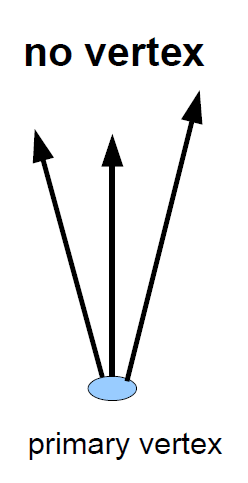
\includegraphics[width=\textwidth]{Figures/jetClasses/class1.png}
%%     \caption{}
%%     \label{fig:class1}
%%   \end{subfigure}~
%%   \begin{subfigure}[H]{0.2\textwidth}
%%     \centering
%%     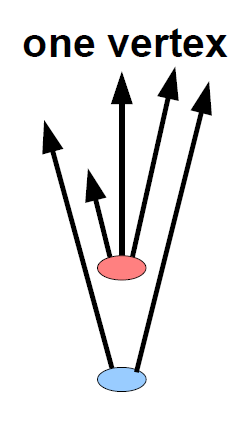
\includegraphics[width=\textwidth]{Figures/jetClasses/class2.png}
%%     \vspace{0.1cm}
%%     \caption{}
%%     \label{fig:class2}
%%   \end{subfigure}~
%%   \begin{subfigure}[H]{0.32\textwidth}
%%     \centering
%%     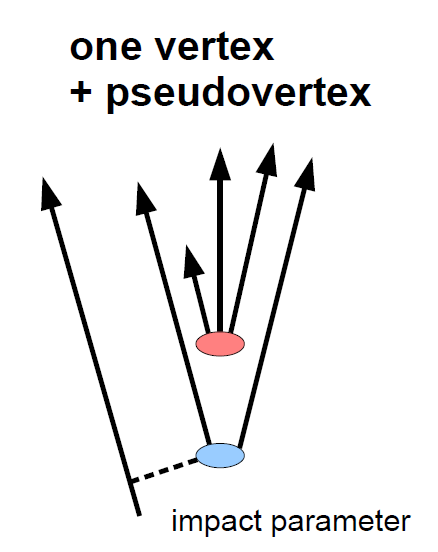
\includegraphics[width=\textwidth]{Figures/jetClasses/class3.png}
%%     \caption{}
%%     \label{fig:class3}
%%   \end{subfigure}~
%%   \begin{subfigure}[H]{0.2\textwidth}
%%     \centering
%%     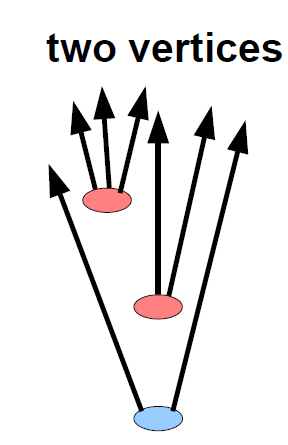
\includegraphics[width=\textwidth]{Figures/jetClasses/class4.png}
%%     \vspace{0.3cm}
%%     \caption{}
%%     \label{fig:class4}
%%   \end{subfigure}
%%   \caption{Schematic of different jet classes, based on the number of secondary vertices.}\label{fig:jetClass}
%% \end{figure}
%% The identification of the flavor of a quark inducing the jets follows the identification of the jet class. Besides the number of secondary vertices, other discriminating \begin{it}input variables\end{it} enter a multivariate discrimination. \\
%% %% After identifying the jet class, we would like to determine the nature of the jets. Of course, for the jet identification we can not only rely on the number of secondary vertices found. It is also needed to study other properties of the jet, for example the mass and other kinematic properties which are called the \begin{it}input variables\end{it}. 
%% For the study reported in this document the LCFIPlus flavor tagging software was used, see also Section \ref{sec:LCFIPlus}. A list of the LCFIPlus input variables is given in \cite{website:LCFIPlus}. For each jet class (Figure \ref{fig:jetClass}), an optimized set of variables is used (see Table \ref{tab:inputVars}). \\
%% The impact parameters $d_0$ and $z_0$ are important parameters used for flavor tagging. The impact parameter of a track is the distance between the tracks's point of closest approach to the IP \cite{Bailey2009573}. The impact parameter $d_0$ gives this distance in the xy-plane and $z_0$ to the z-axis. The \begin{it}significance\end{it} of an impact parameter is the impact parameter divided by its uncertainty. \\
%% A brief explanation for each flavor tag input variable is give below (from \cite{website:LCFIPlus}):
%% \begin{itemize}
%% \item trk1d0sig/trk2d0sig: d0 significance of track with highest/second highest d0 significance.
%% %\item trk2d0sig: d0 significance of track with second highest d0 significance.      
%% \item trk1z0sig/trk2z0sig: z0 significance of track with highest/second highest d0 significance (ordering by d0, not z0).       
%% %\item trk2z0sig: z0 significance of track with second highest d0 significance (ordering by d0, not z0).
%% \item trk1pt/trk2pt: Transverse momentum of track with highest/second highest d0 significance. 
%% \item trk1pt\_jete/trk2pt\_jete: trk1pt/trk2pt divided by the jet energy.
%% %\item trk2pt: Transverse momentum of track with second highest d0 significance.
%% %\item trk2pt\_jete: trk2pt divided by the jet energy.
%% \item jprobr/jprobz: Joint probability in the r-phi plane/z projection using all tracks.
%% %\item jprobz: Joint probability in the z projection using all tracks.
%% \item vtxlen1\_jete: Decay length of the first vertex in the jet (zero if no vertex is found) divided by the jet energy.
%% \item vtxsig1\_jete: Decay length significance of the first vertex in the jet (zero if no vertex is found) divided by the jet energy. 
%% \item vtxdirang1\_jete: The angle between the momentum (computed as a vector sum of track momenta) and the displacement of the first/second vertex multiplied by the jet energy. 
%% \item vtxmom1\_jete/ vtxmom2\_jete: Number of tracks included in the first vertex (zero if no vertex is found) divided by the jet energy. 
%% \item vtxmass1/vtxmass2: Mass of the first/second vertex computed from the sum of track four-momenta. 
%% \item vtxmult1/vtxmult2: Number of tracks included in the first/second vertex (zero if no vertex is found/number of vertex is less than two). 
%% \item vtxmasspc: Mass of the vertex with minimum $p_T$ correction allowed by the error matrices of the primary and secondary vertices. 
%% \item vtxprob: Vertex probability. For multiple vertices, the probability P is computed as $1-P = (1-P_1)(1-P_2)...(1-P_N)$.
%% \item vtxlen2\_jete: Decay length of the second vertex in the jet (zero if number of vertex is less than two) divided by the jet energy. 
%% \item vtxsig2\_jete: Decay length significance of the second vertex in the jet (zero if number of vertex is less than two) divided by the jet energy. 
%% \item vtxdirang2\_jete: The angle between the momentum (computed as a vector sum of track momenta) and the displacement of the second vertex multiplied by the jet energy.
%% %\item vtxmom2\_jete:      
%% %\item vtxmass2          
%% %\item vtxmult2          
%% \item vtxlen12\_jete: Distance between the first and second vertex (zero if number of vertex is less than two) divided by the jet energy. 
%% \item vtxsig12\_jete: vtxlen12 divided by its error as computed from the sum of the covariance matrix of the first and second vertices, projected along the line connecting the two vertices divided by the jet energy. 
%% \item vtxdirang12\_jete: The angle between the two vectors as defined as follows. The first vector is the displacement vector from vertex 1 to vertex 2. The second vector is the difference of the vertex momentum 1 and vertex momentum 2. The computed angle is then normalized by the jet energy.
%% \item vtxmom\_jete: The vertex momentum normalized by the jet energy, where the vertex momentum is computed by simply summing the momentum of tracks used to create vertices. If there are multiple vertices they are simply added. 
%% \item vtxmass: Vertex mass as computed from the sum of four momenta of all tracks forming secondary vertices. 
%% \item vtxmult: Number of tracks which are used to form secondary vertices (summed for all vertices). 
%% \item 1vtxprob: Vertex probability with all tracks associated in vertices combined.
%% \item jprobr5sigma/jprobz5sigma: Joint probability in the r-$\phi$ plane/z projection using all tracks having impact parameter significance exceeding 5 sigma.
%% \item d0bprob/d0cprob/d0qprob: Product of b/c/q-quark probabilities of $d_0$ values for all tracks, using b, c, q $d_0$ distributions.
%% \item z0bprob/z0cprob/z0qprob: Product of b/c/q-quark probabilities of $z_0$ values for all tracks, using b, c, q $z_0$ distributions.
%% \item trkmass: Mass of all tracks exceeding 5 sigma significance in $d_0/z_0$ values.
%% \end{itemize}

%% \begin{table}[b]
%%  \caption{LCFIPlus input variables used for different jet classes. The variables in blue are added to the input variables during this project.} 
%%   \begin{center}
%%   \begin{tabular}{|c|c|c|c|}
%%     \hline
%%     Category 1   & Category 2       & Category 3        & Category 4        \\ \hline \hline
%%     trk1d0sig    & trk1d0sig        & trk1d0sig         & trk1d0sig         \\       
%%     trk2d0sig    & trk2d0sig        & trk2d0sig         & trk2d0sig         \\       
%%     trk1z0sig    & trk1z0sig        & trk1z0sig         & trk1z0sig         \\       
%%     trk2z0sig    & trk2z0sig        & trk2z0sig         & trk2z0sig         \\       
%%     trk1pt\_jete & trk1pt\_jete     & trk1pt\_jete      & trk1pt\_jete      \\       
%%     trk2pt\_jete & trk2pt\_jete     & trk2pt\_jete      & trk2pt\_jete      \\        
%%     \textcolor{blue}{jprobr5sigma} & jprobr           & jprobr            & jprobr            \\       
%%     \textcolor{blue}{jprobz5sigma} & jprobz           & jprobz	        & jprobz            \\        
%%     \textcolor{blue}{d0bprob}      & \textcolor{blue}{d0bprob}          & vtxlen1\_jete     & vtxlen1\_jete     \\        
%%     \textcolor{blue}{d0cprob}      & \textcolor{blue}{d0cprob}          & vtxsig1\_jete     & vtxsig1\_jete     \\         
%%     \textcolor{blue}{d0qprob}      & \textcolor{blue}{d0qprob}          & vtxdirang1\_jete  & vtxdirang1\_jete  \\            
%%     \textcolor{blue}{z0bprob}      & \textcolor{blue}{z0bprob}          & vtxmom1\_jete     & vtxmom1\_jete     \\         
%%     \textcolor{blue}{z0cprob}      & \textcolor{blue}{z0cprob}          & vtxmass1          & vtxmass1          \\       
%%     \textcolor{blue}{z0qprob}      & \textcolor{blue}{z0qprob}          & vtxmult1          & vtxmult1          \\       
%%     \textcolor{blue}{trkmass}      & vtxlen1\_jete    & vtxmasspc         & vtxmasspc         \\       
%%                  & vtxsig1\_jete    & vtxprob           & vtxprob           \\       
%%                  & vtxdirang1\_jete & 1vtxprob          & vtxlen2\_jete     \\       
%%                  & vtxmom1\_jete    & vtxlen12all\_jete & vtxsig2\_jete     \\             
%%                  & vtxmass1         & vtxmassall        & vtxdirang2\_jete  \\       
%%                  & vtxmult1         &                   & vtxmom2\_jete     \\       
%%                  & vtxmasspc        &                   & vtxmass2          \\       
%%                  & vtxprob          &                   & vtxmult2          \\       
%%                  & \textcolor{blue}{trkmass}          &                   & vtxlen12\_jete    \\ 
%%                  &                  &                   & vtxsig12\_jete    \\ 
%%                  &                  &                   & vtxdirang12\_jete \\ 
%%                  &                  &                   & vtxmom\_jete      \\ 
%%                  &                  &                   & vtxmass           \\ 
%%                  &                  &                   & vtxmult           \\ 
%%                  &                  &                   & 1vtxprob          \\ \hline

%%   \end{tabular}
%%   \end{center}
%%   \label{tab:inputVars}
%% \end{table}
